% !Mode:: "TeX:UTF-8"
%此为第一章节。
%\figure为图片,[h]为hear代码所在,\caption为表名图名,\includegraphics为引用位置,\cite为引用参考文献,\begin{equation}公式,\subfloat子图,\label标签,\begin{table}表格,\begin{tabular}三线表,{cccc}完全居中,\toprule,\multirow取几行,\cmidrule取第几列\begin{theorem}定理,\begin{proof}证明,\begin{corollary}推论,\begin{lemma}引理
    
\chapter{绪\quad 论}
\section{研究工作的背景与意义}

\begin{shaded}
    微电子器件整体发展趋势  
    \end{shaded}
    随着人工智能和第五代移动通信技术等系统技术的发展,推动着半导体行业在移动便携设备、高性能计算机、自动驾驶、物联\cite{lau_recent_2022}网和大数据等应用领域的发展\cite{lau_recent_2022},同时也推动着电子芯片向着小型化和高集成化方向发展快速发展\cite{sadique_heat_2022}。在过去的几十年里处理器上的晶体管数量依照这摩尔定律\cite{moore_cramming_1965}的预测呈现出指数级的增长趋势,如\cref{chip-develop}所示。摩尔定律与登纳德定律\cite{dennard_design_1974}引领着半导体行业飞速发展,半导体芯片上电子元件的数量与日俱增,大大提高了芯片的综合性能。随着半导体芯片性能的提高,以及尺寸的限制,导致芯片工作时温度的急剧上升,这将对其正常的运行工作产生严重的影响。半导体芯片散热器技术的发展已成为制约半导体芯片进一步发展的一大重要原因。

    \begin{figure}[h]
        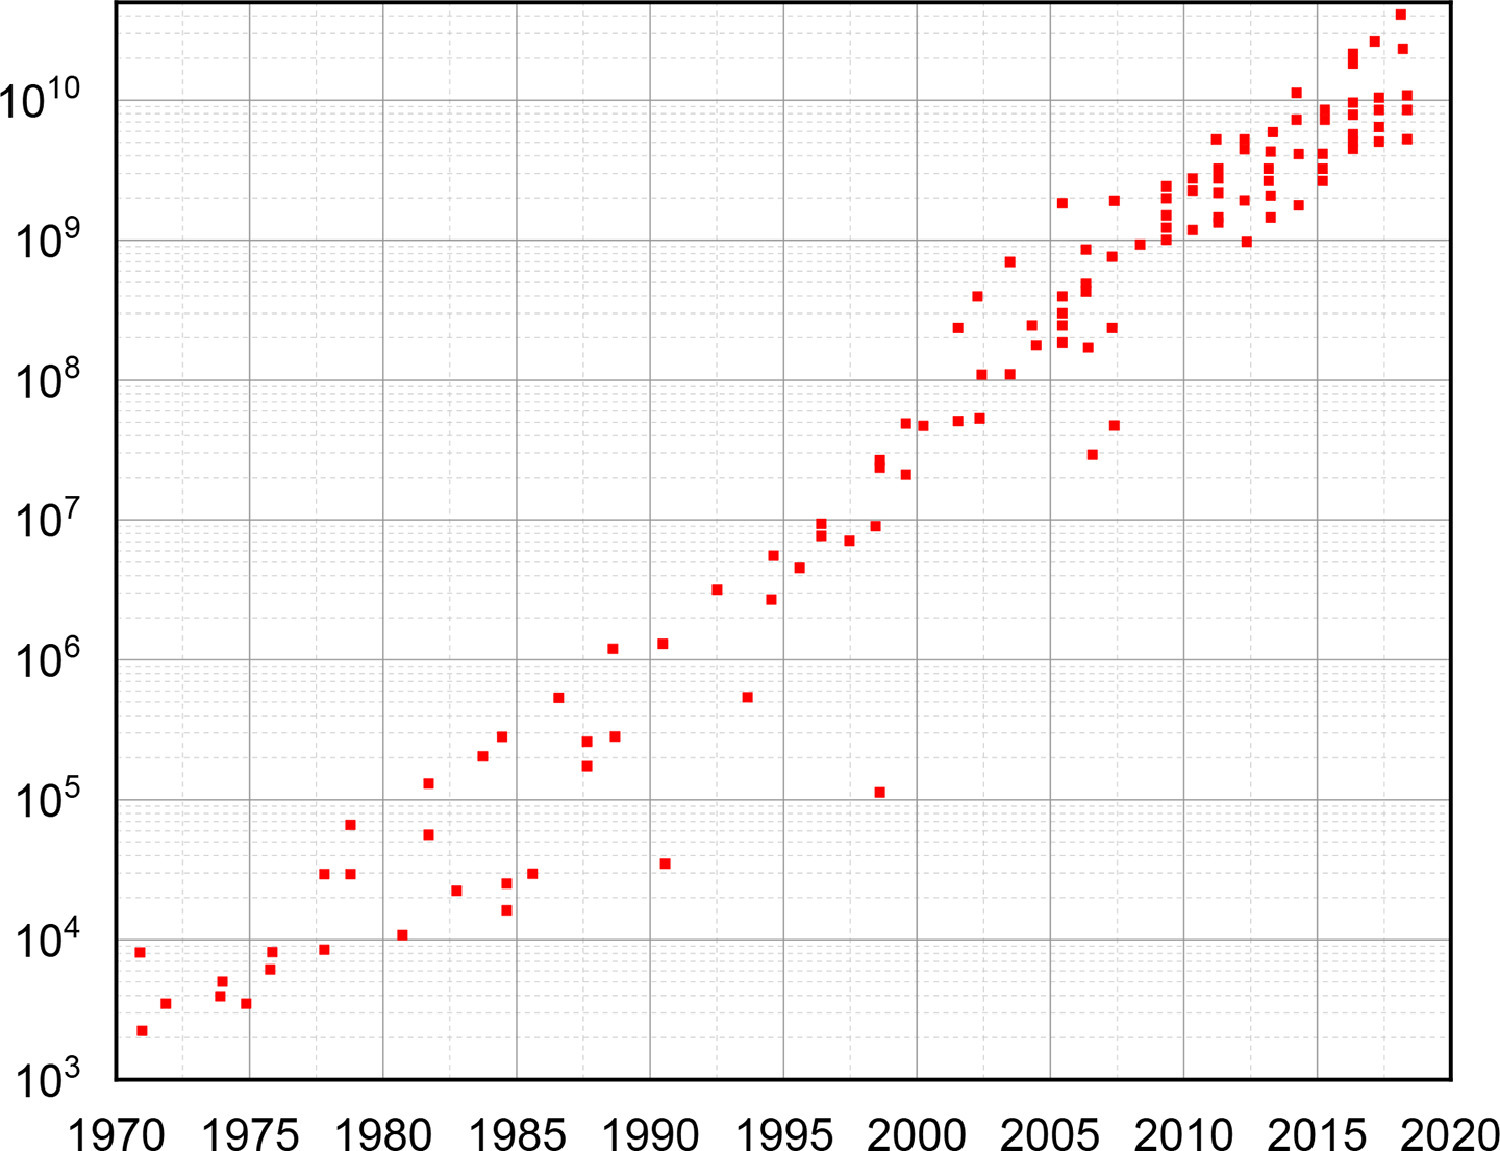
\includegraphics[width =0.5\linewidth]{chip-develop.jpg}
        \caption{半导体芯片上的晶体管数量}
        \label{chip-develop}
        \end{figure}


    \begin{equation}
        MTF = \frac{1}{{A{J^2}}}{\rm{exp}} - \frac{\phi }{{{K_B}T}}
        \label{MTF}
        \end{equation}



本论文以时域积分方程时间步进算法的数值实现技术、后时稳定性问题以及两层平面波加速算法为重点研究内容,主要创新点与贡献如下:

        \begin{algorithm}[H]
            \KwData{this text}
            \KwResult{how to write algorithm with \LaTeX2e}
            initialization\;
            \While{not at end of this document}{
                read current\;
                \eIf{understand}{
                    go to next section\;
                    current section becomes this one\;
                }{
                    go back to the beginning of current section\;
                }
            }
            \caption{How to wirte an algorithm.}
        \end{algorithm}

